\chapter{Online Learning}\label{ch:OnlineLearning}

Online Learning is a theoretical framework to formalize a sequential decision problem in which an agent has to take consecutive actions in an environment. Every time the agent takes an action, the environment returns a loss signal (or reward depending on the sign convention). This framework is similar to other sequential decision problems such as Reinforcement Learning \cite{sutton2018reinforcement}, with the main difference that in Online Learning there isn't a concept of transition probability from one state to another.
The purpose of this section is to present the general framework of Online Game Playing and to introduce the notation necessary for the development of the theory for Online Portfolio Optimization. We define formally the framework of Online Learning with Expert Advice, which is one of the most studied frameworks of Online Learning, due to its ability to include many other frameworks, such as Multi Armed Bandit \cite{bubeck2012regret} or Online Convex Optimization \cite{hazan2016introduction}.
Then we present the concept of \emph{Regret} and the relationship of Online Learning to classical repeated games, a classical framework coming from the field of Game Theory. 
We are interested in this framework in order to model repeated investments.
Modern finance has more and more the need for a Game Theoretic approach, which is evident when looking at the field of \emph{On-venue Market Making}, that can be modeled naturally as a repeated game, or of \emph{Merger and Acquisition} that can be modeled as a normal-form game \cite{Yanqing_MaA}.\footnote{For example, Jane Street (one of the biggest players in providing liquidity to the markets) gives extensive training in game theory for its employees.} In addition we think these methods are a viable option to cope with the unknown non-stationary nature of the financial markets.
Finally, we introduce Online Convex Optimization as a special case of Online Learning with expert advice and we show its interesting relationship to theoretical statistical learning. The choice of this path, from Online Learning to Online Convex Optimization, has been done to show how general and powerful Online Learning is in its simplicity, and why Online Convex Optimization is the most suitable framework to present our contribution to Online Portfolio Selection, a framework that will be presented in Chapter \ref{ch:OPO}.

Indeed, even if we focus on the portfolio problem, the apparently simple formulation of this framework is capable to encompass many other applications and problems, such as network routing~\cite{belmega2018online}, dark pool order allocation~\cite{agarwal2010optimal}, e-commerce pricing (\cite{trovo2015multi}, \cite{trovo2018improving}, \cite{paladino2017unimodal}) and advertisement (\cite{gasparini2018targeting}, \cite{nuara2018combinatorial}, \cite{nuara2020online}, \cite{nuara2019dealing}, \cite{gatti2015truthful}).
Moreover Online Learning has also been applied to the Game Theory field of \emph{Security Games} (\cite{jiang2013game}, \cite{bisi2017regret}).
A thorough dissertation of the techniques that have been developed in the field of Online Learning can be found in \cite{cesa2006prediction}.

\section{Online Learning}
\label{sec:OnlineLearning}
% \begin{definition}(Online Game Playing).\label{def:OGP}
%     Let $\mathcal Y$ be the outcome space, $\mathcal D$ the prediction space and $f:\mathcal D\times\mathcal Y\to \mathbb R$ is a loss function, an Online Game is the following sequential game played by the forecaster $\mathcal A$ and the environment:

%     For each round $t\in \mathbb N$
%     \begin{enumerate}
%         %\item Each expert $E_i\in\mathcal E$ choose its prediction $x_{t,E_i}\in\mathcal D$
%         \item The learner $\mathcal A$ chooses an element of the decision space $x_t\in\mathcal D$.
%         \item The environment chooses the element $y_t\in\mathcal Y$, and subsequently determines the loss function $f(\cdot,y_t)$.
%         \item The agent $\mathcal A$ incurs in a loss $f(x_t,y_t)$.
% 		\item The agent updates its cumulative losses $L_t=L_{t-1}+f(x_t,y_t)$ with $L_0=0$.
%     \end{enumerate}
% \end{definition}\todo{F: algorithm. M: si, mi piace. Ma dentro alla definizione un algo?}
% =======

\begin{definition}(Online Learning).\label{def:OGP}
    Let $\mathcal Y$ be the outcome space, $\mathcal D$ the prediction space, and $f:\mathcal D\times\mathcal Y\to \mathbb R$ is a loss function, an Online Game is the sequential game played by the forecaster $\mathcal A$ and the environment, described in Algorithm \ref{alg:OL}.
\end{definition}

\begin{algorithm}[ht!]
    \caption{Online Learning} 
    \label{alg:OL}
    \begin{algorithmic}[1]
    \REQUIRE Decision space $\mathcal D$, outcome space $\mathcal Y$, loss function $f:\mathcal D\times\mathcal Y\to\mathbb R$ \nonumber
    \STATE Set $L_0=0$
    \FOR {$t \in \mathbb R^N$}
    \STATE The learner $\mathcal A$ chooses an element of the decision space $x_t\in\mathcal D$
    \STATE The environment chooses the element $y_t\in\mathcal Y$, and subsequently determines the loss function $f(\cdot,y_t)$
    \STATE The agent $\mathcal A$ incurs in a loss $f(x_t,y_t)$
    \STATE The agent updates its cumulative losses $L_t=L_{t-1}+f(x_t,y_t)$
    \ENDFOR
    \end{algorithmic}
\end{algorithm}
% =============


In Online Learning an agent $\mathcal A$ has to guess the outcome $y_t$ based on the past sequence $y_1,y_2,\ldots,y_{t-1}$ of events that are in the outcome space $\mathcal Y$, at each time step the agent will play (sometimes we will also say \emph{predict}) $x_t$, that is an element of the prediction space $\mathcal D$, and the environment will choose a loss function $f(\cdot,y_t)$ by determining the outcome $y_t$.
The agent $\mathcal A$ is essentially the identification of the functions that map the history of past outcomes to the new prediction:
$$\mathcal A\equiv\left\{h_{t-1}:=(y_1,\ldots,y_{t-1})\longmapsto x_t\right\}_{t\ge 1}. $$
The simplest case is for $\mathcal Y=\mathcal D$ and both of finite cardinality, meaning that there are only a finite number of actions that the agent $\mathcal A$ can choose from.

We will sometimes refer to the environment defined in Section \ref{def:OGP} as ``adversarial'', since no stochastic characterization is given to the outcome sequence $y_t$ and the analysis of the regret is done assuming a worst case scenario.
Since the adversary knows the prediction $x_t$ before deciding the outcome $y_t$, designing an algorithm which tries to minimize the loss is an hopeless task and so we have to set an easier scope. In Section \ref{sec:regret_and_experts} we will also present the counterexample that explains why the absolute minimization of the loss is an hopeless task, and show the suitable framework for successful Online Learning in Adversarial Environment.

% ==================================================

% The assumption\todo{Non qui} of a model for the data even existing is basically assuming the stationarity of the observed events. This may be reasonable in some cases, like speech recognition in which we can assume that there is constant model which translate sound of speech into its lexical transliteration, but it not as reasonable in other cases, as trivial as spam filtering. In email classification for spam filtering, the spam writers actually adapts to the filter itself and every constant model would eventually be out of fashion after some time. In such a regime you need a way of adapting your hypotheses during the learning procedure. This is were Online Learning comes to help. In Online Learning we do not make any assumption on the structure of the data and constantly adapting our hypothesis in order to asymptotically perform as the best hypothesis in hindsight.

% =================================================

\subsection{Regret and Experts}\label{sec:regret_and_experts}
\begin{figure}[!ht]
\centering
\begin{pspicture}(0,-3.42)(8.18,3.42)
\psframe[linecolor=black, linewidth=0.04, dimen=outer, framearc=0.1](6.54,0.9)(2.78,-0.36)
\psframe[linecolor=black, linewidth=0.04, dimen=outer, framearc=0.1](6.52,3.42)(2.82,2.3)
\rput[bl](3.76,2.7){Agent: $\mathcal A$}
\rput[bl](3.68,0.12){Environment}
\psline[linecolor=black, linewidth=0.036, arrowsize=0.05291667cm 2.0,arrowlength=1.4,arrowinset=0.0]{->}(6.54,2.8)(7.66,2.8)(7.66,0.2)(6.54,0.22)
\rput[bl](7.9,1.44){$x_t$}
\psline[linecolor=black, linewidth=0.036, arrowsize=0.05291667cm 2.0,arrowlength=1.4,arrowinset=0.0]{->}(2.78,0.3)(1.46,0.3)(1.46,2.88)(2.8267796,2.8677726)
\rput[bl](0.0,1.2){$f(x_t,y_t)$}
\psframe[linecolor=black, linewidth=0.036, dimen=outer, framearc=0.1](6.2,-2.2)(3.16,-3.42)
\rput[bl](3.78,-2.92){Experts: $\mathcal E$}
\rput[bl](2.96,-1.36){$x_{e,t}$}
\rput[bl](5.26,-1.34){$f(x_{e,t},y_t)$}
\psline[linecolor=black, linewidth=0.036, arrowsize=0.05291667cm 2.0,arrowlength=1.4,arrowinset=0.0]{->}(3.8,-2.22)(3.8,-0.36)
\psline[linecolor=black, linewidth=0.036, arrowsize=0.05291667cm 2.0,arrowlength=1.4,arrowinset=0.0]{->}(5.18,-0.4)(5.18,-2.22)
\end{pspicture}

\caption{Online Learning with Expert Advice as Multi Agent-Environment interaction.}
\label{fig:OL}
\end{figure}

We stated that the objective of absolute loss minimization is hopeless in an adversarial framework, as the adversary can always choose the outcome $y_t$ that maximizes the loss $f(x,y_t)$ regardless of the decision $x\in\mathcal D$ taken by the learner. More formally, assume $\mathcal D$ to be the space of binary outcomes, \emph{i.e.}, $|\mathcal D|=2$, and that $f$ is the absolute loss $f(x,y)=|x - y|$. Since the adversary plays after the learner $\mathcal A$, it can  make the loss of the learner $L_T=T$ by choosing $y=1-x$ as the bit non predicted by the learner, making $f(x,y)=1$ at each time step. Notice that no assumption has been made on the strategy followed by the learner $\mathcal A$.
From this example it is clear that the learner has to set a less ambitious goal.

We do so by extending the theoretical formulation in Section \ref{sec:OnlineLearning} by including a set $\mathcal E$ of other players, this setting is called \emph{prediction with expert advice}. At each time step of the prediction game, each expert $e\in\mathcal E$ predicts an element $x_{e,t}\in\mathcal D$, and incurs in a loss $f(x_{e,t},y_t)$, just as the agent $\mathcal A$, creating a general multi-agent interaction as in Figure~\ref{fig:OL}. 
The goal of the learner is to obtain small losses with respect to the best expert in the class $\mathcal E$. This concept is captured by the definition of regret.
Formally, we define the regret $R_{e,T}$ for the agent $\mathcal A$ with respect to expert $e\in\mathcal E$ as follows:

\begin{equation}\label{def:Regret}
	R_{e,T} = L_T-L_{e,T}.
\end{equation}

The regret observed by the agent $\mathcal A$ with respect to the entire class of experts $\mathcal E$ is defined as:

\begin{equation}
	R_T=\sup\limits_{e\in\mathcal E}R_{e,T}=L_T-\inf\limits_{e\in\mathcal E}L_{e,T}.
\end{equation}

The task agent $\mathcal A$ is to find a sequence $x_t$, function of the information obtained up to the time $t$ in order to obtain small regret $y_T$ with respect to any sequence $y_1,y_2,\ldots$ chosen by the environment.

In particular we aim to achieve sub-linear regret $R_T= o(T)$, meaning that the per-round regret $R_T/T$ will asymptotically vanish: 

\begin{equation}
	R_T= o(T) \implies \lim\limits_{T\to \infty}\frac{R_T}{T}=0,
\end{equation}

where $ o(T)$ is the space of sub-linear affine functions. A strategy $\mathcal A$ that attains sub-linear regret is called \emph{Hannan-Consistent}~\cite{hannan1957approximation}.

The regret is a measure of the distance between our online performance and the best offline (in retrospect) performance among the expert class $\mathcal E$, which is also called \emph{external regret} since it is compared to the external set of experts $\mathcal E$. A surprising fact is that such algorithms do even exist.
Indeed a first result is that \emph{in general} there are no Hannan-consistent strategies, and just introducing the concept of regret is not enough by itself for successful Online Learning. 

A first simple counterexample can be found in~\cite{cover1966behavior}. If the decision space $\mathcal D$ is finite, then there exists a sequence of loss function such that $R_T=\Omega(T)$.
% Cover Impossibility
Again take $\mathcal D$ as a space of binary outcomes, absolute loss as $f(x,y)=|x - y|$, and the class of experts is composed by two experts, one predicting always $0$ and the other always $1$. Taking $T$ odd, we have that the loss of the best expert is $L_{e,T}<\frac{T}{2}$, and we have already shown that the adversary can make the loss of the learner $L_T=T$. It is now evident that the regret is $R_T>T-\frac{T}{2}$, which does not allow $R_T/T\to 0$. This argument is easily extended in the case of any finite decision space $\mathcal D$.

To achieve sub-linear regret, the learner has to randomize its predictions, and, at each turn $t$, the agent choose a probability distribution on the decision space and plays $x_t$ according to this distribution. Clearly the adversary has knowledge of the probability distribution of the learner $\mathcal A$, but has no knowledge of the random seed used by the agent $\mathcal A$, \emph{i.e.}, does not know the actual decision sampled from the distribution held by the agent. If the original decision space was $\mathcal D$, with $|\mathcal D|=N$, after the randomization of the decision, we effectively transformed the decision space $\mathcal D$ into the $\Delta_{N-1}\in\mathbb R^{N}$ probability simplex. By doing so we are formally extending the game into its mixed extension, as will be discussed further in Section \ref{sec:GT}. It can be viewed also as a \emph{covexification} of the domain, pointing to the undeniably necessity of convex geometry in this context, that will be discussed in Section \ref{sec:OCO}. Therefore, from now on the domain $\mathcal D$ will be convex, either by the problem specification or by randomized convexification if the problem has a discrete decision space.

\subsection{Existence of No-Regret Strategies}\label{sec:existence_of_no_regret}
In this section we will show the existence of Hannan-consistent strategies in the case of finite experts and provide a general form to generate sub-linear regret strategies. 
The general idea with a finite class of experts is given by the Weighted Average Forecaster, which implements the natural idea of playing as the weighted average of the experts predictions:

\begin{definition}(Weighted Average Forecaster).\label{def:weighted_avg}
For a finite class of experts $\mathcal E=\{E_1,\ldots,E_N\}$, the weighted average prediction is defined as:
\begin{equation}
	x_t = \frac{\sum\limits_{i=1}^{N}w_{i,t-1}x_{i,t}}{\sum\limits_{i=1}^{N}w_{i,t-1}},
\end{equation}
where $w_{i,t-1}>0$, and $x_{i,t}$ is the prediction of expert $E_i\in\mathcal E$ at round $t$. 
\end{definition}

Since $\mathcal D$ is convex we have that $x_t\in\mathcal D$.
Then it is natural to assume that the weights are a function of the cumulated regret suffered by the agent with respect to the experts, and also that the change in weight is proportional to the change in a potential function.
We can generalize the simple weighted average prediction in Equation \eqref{def:weighted_avg} in the following general form, introduced in~\cite{cesa2003potential}:

\begin{equation}\label{eq:potential_avg}
x_t = \frac{\sum\limits_{i=1}^{N}\partial_i \Phi(\mathbf R_{t-1}) x_{t,i}}{\sum\limits_{i=1}^{N}\partial_i \Phi(\mathbf R_{t-1}) },
\end{equation}

where $\Phi(\mathbf u)=\varphi\left(\sum\limits_{i=1}^N\phi(u_i)\right)$ is a function $\Phi:\mathbb R^N\to\mathbb R^+$ defined through two increasing functions $\phi,\varphi:\mathbb R\to\mathbb R^+$, $\varphi,\phi\in\mathcal C^2(\mathbb R)$ concave and convex, respectively, and $\mathbf R_T=(R_{1,T},\ldots,R_{N,T})$.
By specializing the two functions $\varphi,\phi$ we can derive a large class of the algorithms for dealing with prediction under expert advice.
The reasons behind the general form of Equation \eqref{eq:potential_avg} are quite complex and an extended discussion can be found in~\cite{hart2001general}, \cite{cesa2003potential} and \cite{blackwell1956analog}, but the general idea is that the form of Equation \eqref{eq:potential_avg} has the following property:

\begin{theorem}\cite{cesa2003potential}
	If $x_t$ is given by Equation~\eqref{eq:potential_avg} and the loss $f(\cdot,y)$ is convex in the first argument, then the instantaneous weighted regret satisfies:  
	$$\sup\limits_{y_t\in\mathcal Y}\sum\limits_{i=1}^N[f(x_t,y_t)-f(x_{i,t},y_t)]\partial_i \Phi(\mathbf R_{t-1}) \le 0.$$
\end{theorem}

\begin{proof}
	By convexity of $f(\cdot,y_t)$ we have that:
\begin{align}\label{eq:blw_cond}
	f(x_t,y_t)\le\frac{\sum\limits_{i=1}^N\partial_i\Phi(\mathbf R_{t-1})f(x_{i,t},R_t)}{\sum\limits_{i=1}^N\partial_i\Phi(\mathbf R_{t-1})}, \forall y_t\in\mathcal Y.
\end{align}
And since $\Phi(\mathbf x)=\varphi\left(\sum\limits_{i=1}^N \phi(x_i)\right)$ we have that:
$$\partial_i\Phi(\mathbf x)=\varphi'\left(\sum\limits_{i=1}^N\phi(x_i)\right)\phi'(x_i)\ge0.$$
Hence, we can rearrange the terms in Equation~\eqref{eq:blw_cond} to obtain the statement.
\end{proof}

Note that fixing the structure for the weights as in Equation \eqref{eq:potential_avg} we have that $w_{t,i}\propto\phi'(R_{i,t})$ is an increasing function in $R_{i,t}$ (since $\phi$ is convex and increasing) that essentially states that we are increasing the probability of playing actions on which we saw large regret $R_{i,t}$.

\begin{definition}(Exponentially Weighted Algorithm)\label{def:ewf}
	The Exponentially weighted algorithm is obtained from Equation \eqref{def:weighted_avg} by defining:
	\begin{equation}\label{eq:weights_ewf}
	w_{i,t-1}=e^{\eta R_{i,t-1}}/\sum\limits_{j=1}^Ne^{\eta R_{j,t-1}}.
	\end{equation}
\end{definition}

Note that, the exponentially weighted algorithm is also Equation \eqref{eq:potential_avg} where we defined $\varphi(x)=\frac{1}{\eta}ln(x)$ and $\phi(x)=e^{\eta x}$ giving weights defined in Equation \eqref{eq:weights_ewf}.

It can be shown (\cite{cesa2006prediction} Theorem 2.2) that the algorithm defined by the update rule in Equation \eqref{def:ewf}, and for a convex loss function $f(\cdot,y_t)$, gives the following guarantee on the regret:
\begin{equation}\label{eq:regret_ewf}
R_T\le \frac{log(N)}{\eta}+\frac{T\eta}{8}.
\end{equation}

By choosing $\eta=O\left(\sqrt\frac{1}{T}\right)$ we obtain a sub-linear regret $R_T=\mathcal O(\sqrt T)$. %It is also possible to make this algorithm an all-time algorithm (no need to know the length of the game $T$, as opposed as a \emph{one-time} algorithm) by using the so called doubling trick by continually adapting the parameter $\eta$. In general a one-time algorithm obtains slightly smaller bounds then the all-time counterparts, that require the knowledge



\section{Experts}
The theoretical framework described in Section \ref{sec:OnlineLearning} is very general and most suited for a game theory analysis of the problem. This helps us to describe many other frameworks, such as Online Optimization \cite{hazan2016introduction}, or Multi Armed Bandit \cite{bubeck2012regret} as embedded into a Game Playing framework with expert advice. It can then be specialized by fixing many elements of the definition, in order to be applied to the specific problem we are willing to solve.
For instance, the class of experts $\mathcal E$ is most of the times completely fictitious, meaning that the experts are not real players of the game but they are \emph{simulable}, meaning that the agent $\mathcal A$ is able to compute $x_{e,t}$ for each expert $e\in\mathcal E$ and most of the times the class of expert is very limited in its actions, \emph{e.g.}, $\mathcal E$ is the class of experts for which $x_{e,t}$ is constant in $t$. In this case, which is the most studied class of experts, we are basically just comparing our learner $\mathcal A$ to the best fixed action $x^*$ in hindsight. This is a clairvoyant strategy that attains the minimum cumulative loss over the entire length of the game $T$.

\subsection{Uncountable Experts}\label{sec:uncountable_exp}

In the case of uncountable experts the Exponentially Averaged Prediction cannot be applied directly, but it can be extended to a continuous mixture of experts predictions. More specifically we need the case of the class $\mathcal E$ being generated by a convex hull of a finite number of a base class of experts, $\mathcal E_N$.
With continuous class of experts $\mathcal E$ defined in this way, the regret definition becomes:

\begin{equation}
    R_T = \sup\limits_{\mathbf q\in\Delta_{N-1}}R_{\mathbf q,T}:=L_T-\inf\limits_{\mathbf q\in\Delta_{N-1}}L_{\mathbf q,T},
\end{equation}

where $\Delta_{N-1}\subset \mathbb R^{N}$ is the $N$-simplex, and 

$$L_{\mathbf q,T}=\sum\limits_{t=1}^T f(\langle \mathbf q,\mathbf x_{e,t}\rangle,y_t),$$
where $\mathbf x_{e,t}=(x_{1,t},\ldots,x_{N,t})\in\mathbb R^N$ is the vector of expert predictions at time $t$.


\section{Exp-Concave loss functions}\label{sec:exp-concave-mixture}

Very important for the study of Portfolio Optimization is the exp-concave class of loss functions. The reason is that the natural loss function used in the Online Portfolio Optimization framework is $1$ exp-concave, as we shall see in Chapter \ref{ch:OPO}.

\begin{definition}(Exp-concave function). 
$g(x)$ is said $\nu$ exp-concave if $e^{-\nu g(x)}$ is concave.
\end{definition}

When speaking about loss functions we are interested in concavity of the function in its first argument. Therefore we will say that a loss function $f$ is $\nu$ exp-concave if $f(\cdot,y)$ is $\nu$ exp-concave $\forall y\in\mathcal Y$. 

\begin{theorem}\label{th:General_Blk}(\cite{cesa2006prediction} Theorem 3.2).
The Exponentially Weighted Average forecaster, for $\nu$-exp concave loss functions, has the following property taking $\eta=\nu$:

$$\Phi(\mathbf R_T)\le \Phi(\mathbf R_0),$$

where $\Phi(x)=\varphi\left(\sum\limits_{i=1}^N\phi(x_i)\right)$ is chosen as $\varphi(x)=\frac{1}{\nu}log(x)$ and $\phi(x)=e^{\nu x}.$

\end{theorem}

\begin{proof}
    The weights are given by $w_{i,t-1}=e^{\nu R_{i,t-1}}/\sum\limits_{j=1}^N e^{\nu R_{j,t-1}}$.
    By exp-concavity we have that:
    \begin{equation}
        e^{-\nu f(x_t,y_t)}=exp\left\{-\nu f \left(\frac{\sum\limits_{i=1}^N w_{i,t-1}x_{i,t}}{\sum\limits_{i=1}^N w_{i,t-1}},y_t\right)\right\}\ge \frac{\sum\limits_{i=1}^N w_{i,t-1}e^{-\nu f(x_{i,t},y_t)}}{\sum\limits_{i=1}^N w_{i,t-1}}.
    \end{equation}
    This can be rewritten as:
    \begin{equation}\label{eq:conc_exp_last}
        \sum\limits_{i=1}^N e^{\nu R_{i,t-1}}e^{\nu [f(x_t,y_t)-f(x_{i,t},y_t)]}\le \sum\limits_{i=1}^N e^{\nu R_{i,t-1}}.
    \end{equation}
    Applying $\varphi(x)=\frac{1}{\nu}log(x)$ to both sides of Equation \eqref{eq:conc_exp_last} we obtain that: 
    $$\Phi(\mathbf R_{t})\le \Phi(\mathbf R_{t-1}),$$ that proves the thesis.
\end{proof}

The case of exp-concave functions is very significant, since thanks to Theorem~\ref{th:General_Blk} we can prove the regret bound for the Exponentially Weighted Average very easily by:

\begin{equation}\label{eq:regret_exp_finite}
    R_T\le \frac{1}{\nu}\log\left(\sum\limits_{i=1}^N e^{\nu R_{j,T}}\right)=\Phi(\mathbf R_T)\le\Phi(\mathbf R_0) = \frac{log N}{\nu}.
\end{equation}

The case of exp-concave losses is also useful for the case of uncountable experts sketched in Section~\ref{sec:uncountable_exp}. This formulation will be of central importance for the portfolio optimization problem.

It is natural to extend the Exponential Weighted Forecaster algorithm described in Definition \eqref{def:ewf} into the case of uncountable expert class $\mathcal E$ generated by the convex hull over the countable class $\mathcal E_N$, by:

\begin{equation}\label{eq:mixture}
    x_t=\frac{\int\limits_{\Delta_{N-1}} w_{\mathbf q,t-1}\langle \mathbf q, \mathbf x_{e,t}\rangle d\mathbf q}{\int\limits_{\Delta_{N-1}} w_{\mathbf q,t-1}d\mathbf q}.
\end{equation}

\begin{theorem}(Mixture forecaster for exp-concave losses)\\
(\cite{cesa2006prediction} Theorem 3.3).\label{th:mixture_forecaster}\\
    Choosing $w_{\mathbf q,t-1}=exp\left\{-\nu\sum\limits_{s=1}^{t-1}f(\langle \mathbf q,\mathbf x_{e,t}\rangle,y_s)\right\}$ in Equation \eqref{eq:mixture}, for a bounded $\nu$-exp concave loss function $f(\cdot,y)$, we obtain:
    $$R_T\le \frac{N}{\nu}\left(log\left(\frac{\nu T}{N}\right)+1\right).$$
\end{theorem}

Even in the case of uncountable many experts, exp-concavity of the loss function gives a better convergence rate of $\mathcal O(\log T)$ then the exponentially weighted algorithm in Equation~\eqref{eq:regret_ewf}, which is $\mathcal O(\sqrt T)$.

% REGRET MINIMIZATION IN GAMES =================================================
\section{Regret Minimization in Games}
\label{sec:GT}
In this section we explore the connection of the framework of Section \ref{sec:OnlineLearning} into a more classical repeated game framework. In the previous section we looked at the adversary as a black box, without any specific model in mind. The reason of this chapter is to clarify its role as a player in the game and to show the game theoretical properties of Hannan-consistent agents. Since in Online Learning the convention is to speak about losses, we shall speak about losses (players are minimizing) also in the classical definitions of game theory instead of payoffs (players are maximizing).

\begin{definition}(Strategic Form $K$-Player Game).\label{def:Game}
    A Strategic form $K$-player game is t a tuple $\langle\mathcal K,\{X_i\}_{i\in\mathcal K},\{l_i\}_{i\in\mathcal K}\rangle$ where:
    \begin{enumerate}
        \item $\mathcal K=\{1,\ldots,K\}$ is the finite set of players.
        \item $X_i$ is the set of actions available to player $i\in\mathcal K$.
        \item $l_i:\bigotimes\limits_{k=1}^KX_i\to\mathbb R$ is the loss observed by player $i\in\mathcal K$.\footnote{we defined $\otimes$ as the Cartesian product.}
    \end{enumerate}
	The game is called finite if $|X_i|<+\infty$ for all $i\in\mathcal K$.
\end{definition}


\subsection{Mixed extension}\label{sec:mixed}
In Section~\ref{sec:OnlineLearning} we saw that it is impossible to obtain sub-linear regret in adversarial environment with finite decision space $\mathcal D$. A first step to solve this has been the \emph{randomized convexification} technique, where finite action spaces are extended into convex sets, given by their probability simplex. Losses are to be interpreted as expected losses when the mixed extension is applied to the formal game. More formally: 

\begin{definition}(Mixed-extension for finite games).
A finite game $\langle\mathcal K,\{X_i\}_{i\in\mathcal K},\{l_i\}_{i\in\mathcal K}\rangle$ can be extended into the game $\langle\mathcal K,\{\tilde X_i\}_{i\in\mathcal K},\{\tilde l_i\}_{i\in\mathcal K}\rangle$, by defining:
\begin{enumerate}
	\item $\tilde X_i=\Delta_{|X_i|-1}\subset \mathbb R^{|X_i|}$ for all $i\in\mathcal K$;
	\item $\tilde l:\bigotimes \tilde X_i\to\mathbb R$ is defined as:
	$$\tilde l(x_1,\ldots,x_K)=\sum\limits_{i_1=1}^N\cdots\sum\limits_{i_K=1}^Np_{i_1}\cdots p_{i_K}l(i_1,\ldots,i_K).$$ 
\end{enumerate}
\end{definition}

Due to the impossibility result of Cover~\cite{cover1966behavior}, we have to work with the mixed extension formulation of the game. So from now on we take this step implicitly.
The taxonomy of game definitions is quite extended and complex, thus we will focus on non-cooperative games \cite{nash1951non} since they are closely related to the setting tacked in the Online Learning field. More specifically, we will need the model for \emph{Zero Sum Game}. 

\begin{definition}($2$-Players Zero-Sum Game).\label{def:ZSG}
A Zero Sum game is a tuple $\langle\{X_1,X_2\},l:X_1\times X_2\to\mathbb R\rangle$. As in Definition~\ref{def:Game} $X_1,X_2$ are the action spaces for Player $1$ (row player) and Player 2 (column player) respectively, and $l(x_1,x_2)$ for $x_i,x_2\in X_1\times X_2$ represents the losses for Player $1$ and profits for Player $2$.
\end{definition}

If this game is played for $T$ turns, we can call it a repeated game, and the losses for each player is defined $L_1^{(T)}=\sum\limits_{t=1}^Tl_i\left(x_i^{(t)},x_2^{(t)}\right)$ and $L_2^{(T)}=-L_1^{(T)}$. 

\subsection{MinMax Consistency}
The field that tries to answer to questions of what guarantees do Hannan-consistent strategies bring to the game theoretical formulation of the problem is referred in literature as \emph{Learning in Games}.
For formal games we can define the \emph{values} for the game as: 
\begin{align}
    V_1=\inf\limits_{x_1\in X_1}\sup\limits_{x_2\in X_2}l(x_1,x_2),\\
	V_2=\sup\limits_{x_2\in X_2}\inf\limits_{x_1\in X_1}l(x_1,x_2).
\end{align}

These are the values that the players can guarantee themselves, meaning that, no matter the strategy of the columns player, the row player could guarantee itself a loss of at maximum $V_2$, the converse holds for the row player. It can be interpreted as the minimum loss (best payoff) that a player could achieve if it knows that the other player would play adversarially. It is clear that $V_2\le V_1$. In the case that the zero-sum-game is a mixed extension of a finite game, then the Von Neumann theorem states that $V_1=V_2$.
 
Now we will embed the framework of Online Game Playing of Section \ref{sec:OnlineLearning} in a two player zero sum game. 
Online Learning is a special form of Zero Sum Game (possibly considering its mixed extension described in Definition \ref{sec:mixed}) where $X_1\equiv \mathcal D$ and $X_2\equiv \mathcal Y$. The loss function $l:X_1\times X_2\to\mathbb R$ can be identified by the loss $f:\mathcal D\times \mathcal Y\to\mathbb R$ of the Online Learning Agent $\mathcal A$.
Now we will explore interesting properties of Hannan-consistent strategies. A surprising fact is that if the row player plays accordingly to a Hannan-consistent strategy then it achieves the value of the game $V_1$. 

\begin{theorem}
    Hannan-consistent agents in Online Game Playing reach asymptotically the minmax value of the one shot game, formally:
    $$\limsup\limits_{T\to +\infty}\frac{1}{T}\sum\limits_{t=1}^Tf(x_t,y_t)\le V.$$
\end{theorem}

\begin{proof}
    Let us suppose that the game is a mixed extension, then from the Von Neumann minmax theorem we have $V=V_1=V_2$.
    Moreover, let us suppose that player $1$ plays an Hannan-consistent strategy and that $y_1,y_2,\ldots \subset \mathcal Y$ is a generic sequence played by the columns player. Then:
    \begin{equation}
        \limsup\limits_{T\to+\infty}\frac{R_T}{T}\le0,
    \end{equation}
    
    can be translated into 
    \begin{equation}\label{eq:second_HC}
        \limsup\limits_{T\to+\infty}\frac{1}{T}\sum\limits_{t=1}^Tf(x_t,y_t)\le\limsup\limits_{T\to+\infty}\frac{1}{T}\inf\limits_{x\in\mathcal D}\sum\limits_{t=1}^Tf(x,y_t).
    \end{equation}

    Let us define $\hat y_T$ as the empirical distribution played by player $2$ up to $T$:
    $$\hat y_T=\frac{1}{T}\sum\limits_{t=1}^Ty_t.$$
    By Equation \eqref{eq:second_HC} we just need to show that $\frac{1}{T}\inf\limits_{x\in \mathcal D} \sum\limits_{t=1}^T f(x,y_t)\le V.$

    This follows from:

    \begin{align}
        \inf\limits_{x\in\mathcal D}\frac{1}{T}\sum\limits_{t=1}^T f(x,y_t)=\inf\limits_{x\in\mathcal D} f(x,\hat y_T)=\sup\limits_{y\in\mathcal Y}\inf\limits_{x\in\mathcal D} f(x,y)\le V,
    \end{align}
    that concludes the proof.
\end{proof}

We showed that regardless of the strategy of player $2$, a player using an Hannan-consistent strategy achieves lower losses than the value of the game $V$. Clearly using an Hannan-consistent strategy means that if player $2$ was not adversarial, then player $1$ could potentially earn a significantly higher average payoff than the value $V$ of the game. By symmetry, if both players play an Hannan-consistent strategy then they will asymptotically reach the value of the game $V$.

\begin{figure}[!ht]
    \centering
    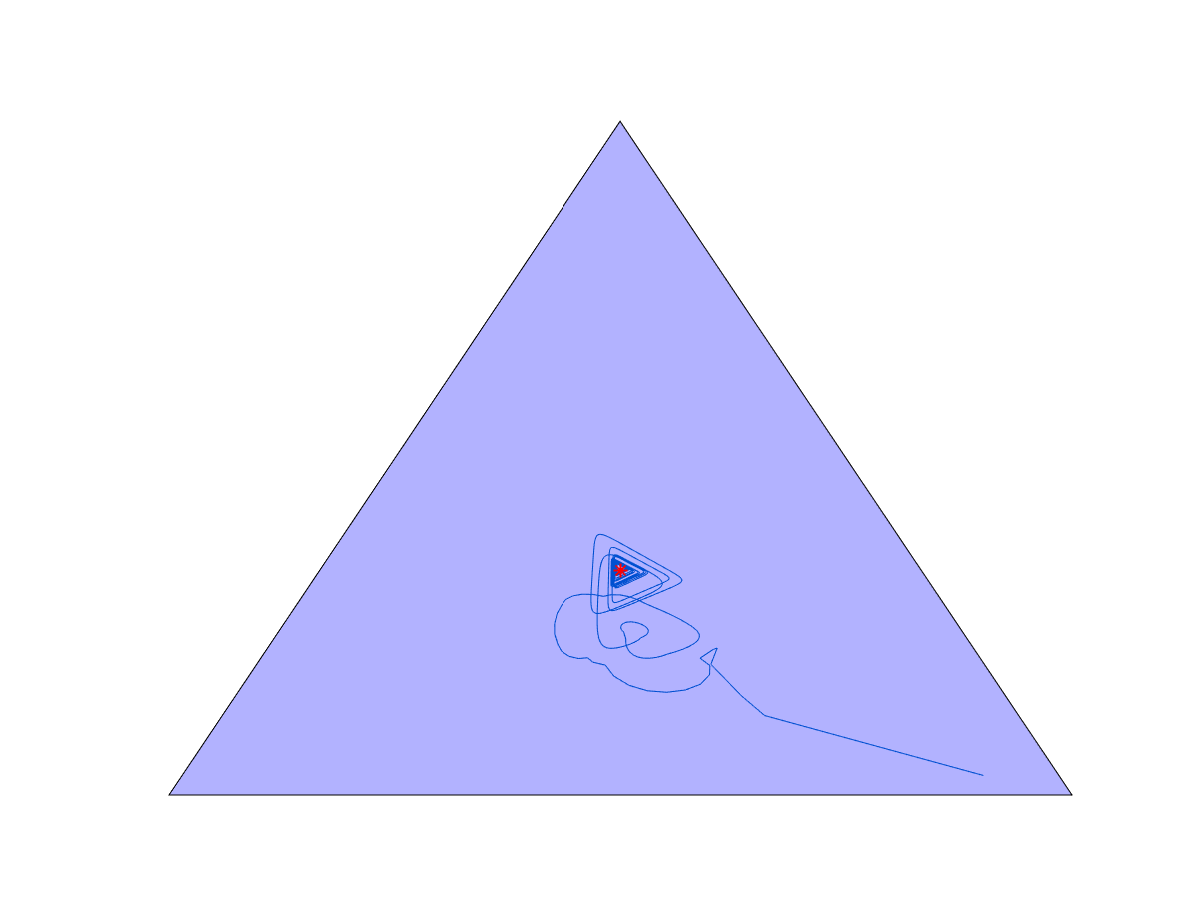
\includegraphics[width=7cm]{./img/rps_ewm.eps}
\caption{Rock Paper Scissor Dynamics in the $\Delta_2$ simplex, generated by the Exponentially Weighted Majority algorithm against an adversarial opponent.}
\label{fig:RPS}
\end{figure}

In Figure \ref{fig:RPS} we present the path of the randomization probabilities of the Rock Paper Scissor game represented in the $\Delta_{2}$ simplex, obtained by the Exponentially Weighted Majority algorithm against an adversarial opponent which plays the best response at each turn, knowing the probabilities of the learner.
Note that the algorithm learns to play the optimal strategy which is the randomization probabilities of $(1/3,1/3,1/3)$ over the action space. 
In general the specific dynamic of policies learned with Hannan consistent strategies are very complex and not well understood \cite{bailey2018multiplicative}.

\section{Online Convex Optimization for Regret Minimization}\label{sec:OCO}

Let us compare this framework to an apparently unrelated problem, namely optimization, that will turn out to be the most suited framework to embed the Online Portfolio Optimization Problem. In online optimization an agent $\mathcal A$ is designed to optimize a sequence of functions $f_t(x)$ where usually $f_t:\mathcal D\to \mathbb R$ is a real valued function from the set $\mathcal D\subset\mathbb R^n$. As a remark on the notation, in Online Convex Optimization literature, the loss functions are written as $f(x,y_t)\equiv f_t(x)$, dropping the explicit dependence on the outcome $y_t$.
The decision space $\mathcal D$ is assumed to be convex, as the functions $f_t:\mathcal D\to \mathbb R$. This framework was first devised in \cite{zinkevich2003online}, and has been later wildly used in the machine learning community to engineer optimization procedures \cite{shalev2012online}. 

Convexity plays a central role in most of the analysis made in Online Learning and Online Convex Optimization. Convexity of the domain $\mathcal D$ and of the loss functions $f(\cdot,y)$ bound the problem geometry and let us derive simple and efficient learning procedures.

In this chapter the decision space $\mathcal D$ is a convex subset of $\mathbb R^N$. As in the case of uncountable experts discussed in Section \ref{sec:uncountable_exp}, the best expert is the one who plays at each round a fixed point $x\in\mathcal D$. In Section \ref{sec:stat_learning} we will discuss how this framework is well suited to optimize complex functions, as Neural Networks, where we can think as $x\in\mathcal D$ as the set of parameters we are trying to optimize. Indeed many state of the art optimization techniques in the field of machine learning have been taking inspiration from the field of Online Optimization \cite{duchi2011adaptive}.

\subsection{A General Algorithm for Online Convex Optimization}\label{sec:OMD}

In this Section we will see an algorithm called \emph{Online Mirror Descent} (OMD), that generalizes many Online Convex Optimization algorithms. It is a first order method (\emph{i.e.}, it uses only information from the gradient of the loss function) that works in the dual space defined by the choice of some regularizator. The OMD algorithm is general and optimal in the sense that every Online Convex problem can be learned online nearly optimally with OMD. The precise definition of the optimality of the OMD algorithm is quite complex to be summarized here and can be found in \cite{srebro2011universality}.
OMD works with a class of regularizators called Bregman Divergences, \cite{banerjee2005clustering}.\footnote{From now on we assume that $\mathcal D\subset \mathbb R^N$ as it is common in the majority of the academic literature on Online Convex Optimization.}

\begin{definition}(Bregman divergence). Given a differentiable convex function $\psi:\mathcal D\to\mathbb R$, the Bregman divergence is defined as an operator $d_{\psi}:\mathcal D\times\mathcal D\to \mathbb R^+$ defined for $\mathbf x,\mathbf y\in\mathcal D\times\mathcal D$ as: 
\begin{equation}\label{eq:bregman_div}
d_\psi(\mathbf x,\mathbf y)=\psi(\mathbf x)-\psi(\mathbf y)-\langle \mathbf x-\mathbf y,\nabla \psi(\mathbf y)\rangle.
\end{equation}
\end{definition}

Since $\psi$ is convex we have that $d_\psi(\mathbf x,\mathbf y)\ge0$. We can see that by linearization of $\psi(\mathbf x)$ around $\mathbf y\in\mathcal D$ and thanks to convexity the other terms are positive. However note that, since the operator defined in Equation \eqref{eq:bregman_div} is not symmetric in its arguments, it does not formally define a metric in the space $\mathcal D$.

Now we will present two example of Bregman divergences that we will use to define specifications of the OMD algorithm in Chapter \ref{ch:algos}.
For $\mathbf x,\mathbf y\in\Delta_{N-1}\subset \mathbb R^N$, consider $\psi(\mathbf x)=||\mathbf x||_2^2$, then the Bregman divergence becomes $d_\psi(\mathbf x,\mathbf y)=||\mathbf x-\mathbf y||_2^2$, which is the Euclidean norm. For $\psi(\mathbf x)=\sum\limits_{i=1}^Nx_i\log(x_i)$ then $d_\psi(\mathbf x,\mathbf y)=\sum\limits_{i=1}^Nx_i\log(x_i/y_i)$, which is the well know Kullback–Leibler divergence~\cite{van2014renyi}.

The OMD algorithm for Online Convex Optimization, described in Algorithm \ref{alg:OMD_in_OCO}, uses the regularization given by a Bregman divergence to follow the best point in the convex set $\mathcal D$ up to now, but it is kept close to the current one by the divergence operator. Formally:

\begin{definition}(Online Mirror Descent). OMD for a Bregman Divergence induced by the differentiable, convex real valued function $\psi$, and for a set of learning rates $\{\eta_0,\ldots,\eta_T\}$ has the following update rule: 

\begin{equation}\label{eq:OMD_update}
\mathbf x_{t+1} =\arginf\limits_{x\in\mathcal D} \left\{d_\psi(\mathbf x,\mathbf x_t)+\eta_t\langle\nabla f_t(\mathbf x_t),\mathbf x-\mathbf x_t\rangle\right\}.
\end{equation}
\end{definition}

Next we will show the idea for a general bound for the OMD algorithm, which explains the geometric ideas behind the OMD algorithm. Note that, in general, the analysis can be refined by fixing the loss function $f_t$ or the convex function $\psi$. \footnote{The convex function $\psi$ is assumed to be differentiable in the domain $\mathcal D$.}

\begin{lemma}\label{th:OMD_first_th}[Theorem 4.1 in \cite{beck2003mirror}].
Let $d_\psi:\mathcal D\times\mathcal D\to \mathbb R$ the Bregman divergence associated to the convex smooth function $\psi$. Moreover, assume $\psi$ is $\alpha$-strong convex w.r.t. $||\cdot||$.
Then $\forall \mathbf x\in\mathcal D$ we have: 
$$\eta_t (f_t(\mathbf x_t)-f_t(\mathbf x))\le d_\psi(\mathbf x,\mathbf x_t)-d_\psi(\mathbf x,\mathbf x_{t+1})+\frac{\eta_t^2}{2}||\nabla f_t(\mathbf x_t)||_*^2,$$ 
\end{lemma}

where we defined the dual norm $||\cdot||_*$ with respect to the norm $||\cdot||$.

\begin{definition}(Dual Norm).
Let $\mathbf x\in X$, the dual norm $||\cdot||_*$ of a norm $||\cdot||$ is defined as:
$$||\mathbf x||_*=\sup\limits_{\mathbf y:||\mathbf y||\le1}\langle \mathbf x,\mathbf y\rangle.$$
\end{definition}

The specific norm $||\cdot||$ in  Theorem \ref{th:OMD_first_th} can be chosen depending on the specific Bregman divergence, in order to simplify the analysis. Indeed, Theorem \ref{th:OMD_first_th} can be used to prove a regret bound for the general OMD algorithm. 

\begin{theorem}(Regret Bound for Online Mirror Descent).\label{th:regret_omd} Together with the assumptions of Theorem \ref{th:OMD_first_th} and if $\eta_t\ge0$ is a decreasing sequence of learning rates, then we have: 
$$R_T\le\max\limits_{t\le T}\frac{d_\psi(\mathbf x,\mathbf x_t)}{\eta_T}+\frac{1}{2\alpha}\sum\limits_{t=1}^T\eta_t||\nabla f_t(\mathbf x_t)||_*^2.$$
\end{theorem}


By choosing $\eta_t=\frac{D\sqrt{\alpha}}{\sqrt{\sum\limits_{t=1}^T||\nabla f_t(\mathbf x_t)||_*^2}}$, where $D=\max\limits_{t\le T}d_\psi(\mathbf x,\mathbf x_t)$, we have a bound for the OMD algorithm of:
\begin{equation}
R_T\le\frac{2D}{\sqrt\alpha}\sqrt{\sum\limits_{t=1}^T||\nabla f_t(\mathbf x_t)||_*^2}.
\end{equation}

Notice that, if the gradient under the dual norm is bounded by $||\nabla f_t(\mathbf x_t)||_*\le G\ \forall t\le T$, then we have that: 
\begin{equation}
R_T\le\frac{2DG}{\sqrt\alpha}\sqrt T,
\end{equation}
which is sub-linear in $T$.

If $\eta_t=\eta>0$ is a constant sequence then Theorem \ref{th:regret_omd} can be simplified to give: 
\begin{equation}
R_T\le \frac{d_\psi(\mathbf x,\mathbf x_1)}{\eta}+\frac{\eta}{2\alpha}\sum\limits_{t=1}^T||\nabla f_t(\mathbf x_t)||^2_*.
\end{equation}

The OMD algorithm is a general technique to exploit the geometric convexity of the problem and gives rise to Hannan-consistent strategies in the case of uncountable convex decision spaces. By specializing the loss function and the Bregman divergences we can generate many algorithms that are state of the art in the Online Convex optimization problem, and achieve better theoretical guarantees than the general analysis we saw for the OMD algorithm. We will show in Chapter \ref{ch:algos} that the Online Newton Step algorithm, even if it can be formulated as an instance of the OMD algorithm, achieves $\mathcal O(\log T)$ regret rather than $\mathcal O(\sqrt T)$ regret.

\begin{algorithm}[t!]
    \caption{Online Mirror Descent for Online Convex Optimization} 
    \label{alg:OMD_in_OCO}
    \begin{algorithmic}[1]
    \REQUIRE learning rate sequence $\{\eta_1, \ldots, \eta_T\}$  \nonumber
    \STATE Set $\mathbf{\mathbf x}_1 \gets \frac{1}{M} \mathbf{1}$ \label{line:init}
    \FOR {$t \in \{ 1, \ldots, T \}$}
    \STATE Observe $f_t(\mathbf x_t)$ decided by the adversary \label{line:out}
    \STATE Set $ g_{t}(\mathbf x)=d_\psi(\mathbf x,\mathbf x_t)+\eta_t\langle\nabla f_t(\mathbf x_t),\mathbf x-\mathbf x_t\rangle$
    \STATE Project $\mathbf x_{t+1} =\arginf\limits_{\mathbf x\in\mathcal D}g_{t}(\mathbf x)$\label{line:update}
    \ENDFOR
    \end{algorithmic}
\end{algorithm}

\subsection{Mirror Version of the Online Mirror Descent Algorithm} \label{sec:mirror_version}

The reason why OMD works is not that we are following the gradient, that points to the minimum of the function; indeed, the sub-gradient (Definition \ref{def:subgradient}) of a loss function does not point to the minimum in general. An example of this phenomena in presented in Figure \ref{fig_no_grad}. In practice the reason why OMD, and other first order methods, are effective is because of the convexity of the loss function and because of the following inequality for the instantaneous regret of convex loss functions:

\begin{figure}[!ht]
\begin{center}
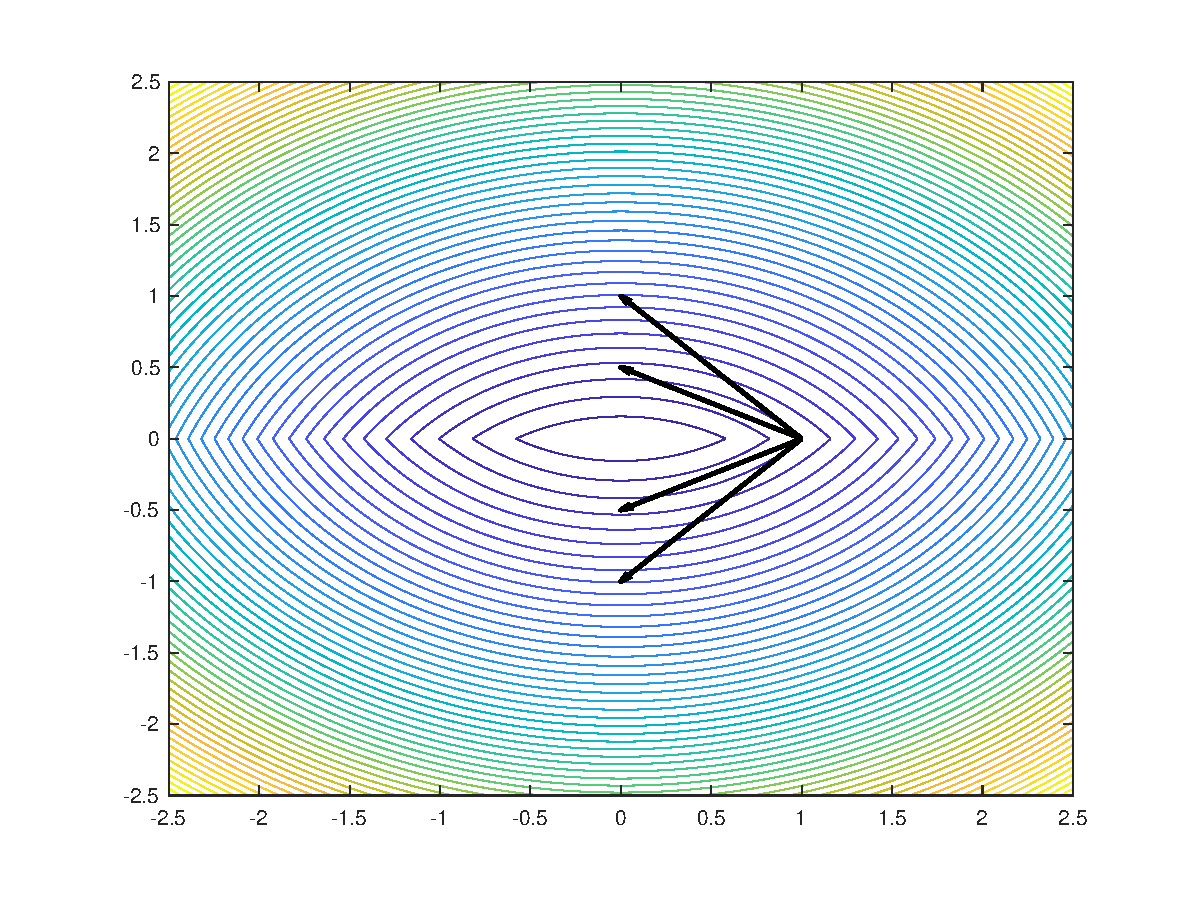
\includegraphics[width=4in,keepaspectratio]{./img/no_grad.eps}
\caption{Contour lines of $f(x,y)=\max\{x^2+(y-1)^2,x^2+(y+1)^2\}$, together with sub-gradient directions from $(1,0)$. All sub-gradient will point to increasing values of the function.}
\label{fig_no_grad}
\end{center}
\end{figure}

\begin{equation}\label{eq:ineq_convex}
f_t(\mathbf x_t)-f_t(\mathbf x)\le\langle\nabla f_t(\mathbf x_t),\mathbf x_t-\mathbf x\rangle,
\end{equation}

and so to minimize the left hand side of Equation \eqref{eq:ineq_convex} we can minimize the right hand side of Equation \eqref{eq:ineq_convex}. Minimizing strictly a linear approximation of the instantaneous regret is not ideal since the environment is adversarial. Instead we minimize the linear approximation together with a regularization term which is given by the Bregman divergence $d_\psi$.

In order to understand more formally the inner workings of the OMD algorithm we have to introduce some concepts from optimization theory:

\begin{definition}(Fenchel Conjugate).\label{def:fenchel_conj}
For a function $f:\mathbb R^N\to\mathbb R$ we can define the Fenchel conjugate as:

\begin{equation}
f^*(\mathbf \theta)=\sup\limits_{\mathbf x\in\mathbb R^N}\langle\mathbf x,\mathbf \theta\rangle -f(\mathbf x).
\end{equation}
\end{definition}

Definition \ref{def:fenchel_conj} can be interpreted as a generalized $\inf$ function as $f^*(\mathbf 0)$ is the classical $\inf$ function. For $\mathbf x\neq\mathbf 0$ then we are looking for the infimum of the function $f$ when the axis of the function are rotated w.r.t. the hyperplane $H(\mathbf x)=\langle\mathbf\theta,\mathbf x\rangle$, as illustrated in Figure \ref{fig:fenchel}. A complete dissertation of the Fenchel duality can be found in \cite{rockafellar1970convex}.

\begin{figure}[!ht]
\centering
\begin{pspicture}(0,-2.4522727)(6.540002,2.4522727)
\psline[linecolor=black, linewidth=0.04, arrowsize=0.05291667cm 2.0,arrowlength=1.4,arrowinset=0.0]{->}(1.7330438,-2.4522727)(1.7330438,2.3477273)
\psline[linecolor=black, linewidth=0.04, arrowsize=0.05291667cm 2.0,arrowlength=1.4,arrowinset=0.0]{->}(0.43304384,-1.5522727)(6.633044,-1.5522727)
\psbezier[linecolor=black, linewidth=0.016](0.033043824,2.0477273)(-0.06695618,-1.5522727)(3.3330438,-1.4522728)(3.3330438,2.0477272727272724)
\psline[linecolor=black, linewidth=0.016](0.43304384,-1.5522727)(4.986615,0.48234266)(5.533044,0.7477273)
\rput[bl](3.5875893,2.1022727){$f(\mathbf x)$}
\rput[bl](5.2603164,0.82045454){$\langle\mathbf x,\mathbf \theta\rangle$}
\psline[linecolor=black, linewidth=0.026](2.317031,-0.42408314)(2.4330437,-0.6522727)
\rput[bl](1.155266,-1.4856061){$\theta$}
\rput[bl](2.233044,-1.0078282){\textcolor{black}{$-f^*(\theta)$}}
\end{pspicture}
\caption{Fenchel Conjugate Function.}
\label{fig:fenchel}
\end{figure}


\begin{definition}(Sub-Gradient).\label{def:subgradient}
For a function $f:\mathbb R^N\to\mathbb R$ we can define the set of sub-differentials at $x_0$ as:
\begin{equation}
\partial f(x_0) = \{g : f(x)-f(x_0) \ge \langle g, x - x_0\rangle,\forall x\}.
\end{equation}
\end{definition}

For a differentiable at $\mathbf x_0$ function we have $\partial f(\mathbf x_0)=\{\nabla f(\mathbf x_0)\}$.

% The two concept clash together in the following theorem:

% \begin{theorem}(\cite{rockafellar1970convex}\label{th:fenchel_subdiff} Theorem 23.5). Let $f:\mathbb R^N\to\mathbb R$ be convex, then:
% \begin{equation}
% \mathbf x\in\partial f^*(\mathbb\theta) \iff \mathbb\theta\in \partial f^*(\mathbf x).
% \end{equation}
% \end{theorem}

% Theorem \ref{th:fenchel_subdiff} is fundamental to prove the following Theorem for OMD:

Finally, the following theorem explains the name of the OMD algorithm and its real more interesting formulation:

\begin{theorem}\label{th:OMD_mirror}
Let $d_\psi$ be a Bregman divergence operator then we have the following equality:

\begin{equation}
\arginf\limits_{\mathbf x\in\mathcal D}\{d_\psi(\mathbf x,\mathbf x_t)+\eta_t\langle\nabla f_t(x_t),\mathbf x-\mathbf x_t\rangle\}=\nabla \psi_{\mathcal D}^*(\nabla \psi(\mathbf x_t)-\eta_t\nabla f_t(\mathbf x_t)),
\end{equation}
where $\psi_\mathcal D$ is the restriction of $\psi$ to the convex set $\mathcal D$, \emph{i.e.,} $\psi_\mathcal D(\mathbf x)=\psi(\mathbf x)+\mathbb I^\infty_\mathcal D(\mathbf x)$, where we defined:
\begin{equation*}
\mathbb I_\mathcal D^\infty(\mathbf x)=\begin{cases}
0&\text{if $\mathbf x\in\mathcal D$}\\
+\infty&\text{otherwise}
\end{cases}.
\end{equation*}
\end{theorem}

% \begin{proof}(Sketch).
% The update rule of Equation \eqref{eq:OMD_update}:
% \begin{align}
% \mathbf x_{t+1}&=\arg\min\limits_{\mathbf x\in\mathcal D}\{d_\psi(\mathbf x,\mathbf x_t)+\eta_t\langle\nabla f_t(x_t),\mathbf x-\mathbf x_t\rangle\}\\
% &=\arg\min\limits_{\mathbf x\in\mathcal D}\langle\eta_t\nabla f_t(\mathbf x_t)-\nabla \psi(\mathbf x_t),\mathbf x\rangle+\psi(\mathbf x),
% \end{align}
% given 
% \end{proof}


Theorem \ref{th:OMD_mirror} shows the real nature of the OMD algorithm, which is to up{}date predictions using the gradient of the loss function, in the dual space defined by the function $\psi$. For example if $\psi(\mathbf x)=\frac{1}{2}||\mathbf x||_2^2$ then we have $\nabla \psi(\mathbf x_t)=\mathbf x_t$ and $\nabla \psi^*(\mathbf x)=\Pi_\mathcal D(\mathbf x)$, and we obtain the Online Gradient Descent algorithm, $\mathbf x_{t+1}=\Pi_\mathcal D(\mathbf x_t-\eta_t\nabla f_t(\mathbf x_t))$, that we will explore with detail in Chapter \ref{ch:OGD}.

\begin{figure}[!ht]
\centering
\begin{pspicture}(0,-2.316111)(8.93147,2.316111)
\psbezier[linecolor=black, linewidth=0.026](4.2682414,-0.4629235)(4.253908,0.08388889)(6.244009,2.449626)(7.3191204,2.017222222222222)(8.394232,1.5848185)(9.182215,0.0771305)(8.653908,-0.7344378)(8.125602,-1.5460061)(5.6539083,-1.4161111)(5.178153,-1.2716666)(4.7023973,-1.1272222)(4.282575,-1.009736)(4.2682414,-0.4629235)
\pstriangle[linecolor=black, linewidth=0.026, dimen=outer](1.5094637,-1.2716666)(3.0,2.6111112)
\psbezier[linecolor=black, linewidth=0.026, arrowsize=0.05291667cm 2.0,arrowlength=1.4,arrowinset=0.0]{->}(1.4539081,0.3838889)(1.8292384,2.1910827)(6.1724277,2.3313398)(6.453908,0.9838888888888868)
\rput[bl](1.2316859,1.2838889){$\mathcal D$}
\rput[bl](3.8094637,2.0061111){$\nabla \psi$}
\psbezier[linecolor=black, linewidth=0.026, arrowsize=0.05291667cm 2.0,arrowlength=1.4,arrowinset=0.0]{->}(5.353908,-0.8161111)(4.6871533,-1.9411111)(1.253908,-2.2161112)(1.253908,-1.0161111111111132)
\rput[bl](3.1205747,-2.316111){$\nabla \psi^*$}
\rput[bl](1.2872415,0.07277778){$\mathbf x_t$}
\rput[bl](1.2316859,-0.88277775){$\mathbf x_{t+1}$}
\rput[bl](6.7101727,0.7838889){$\nabla\psi(\mathbf x_t)$}
\psline[linecolor=black, linewidth=0.026, arrowsize=0.05291667cm 2.0,arrowlength=1.4,arrowinset=0.0]{->}(6.453908,0.8838889)(5.6761303,-0.49388888)
\rput[bl](6.220575,-0.016111111){$\eta_t\nabla f_t(\mathbf x_t)$}
\rput[bl](4.9333954,-0.77508545){$\nabla\psi(\mathbf x_t)-\eta\nabla f_t(\mathbf x_t)$}
\end{pspicture}
\caption{Online Mirror Descent as Mirror Updates.}
\label{fig:OMD_mirror}
\end{figure}

The general procedure for the OMD algorithm is depicted in Figure \ref{fig:OMD_mirror}. We take the past prediction $\mathbf x_t$, we apply the operator $\nabla \psi(\cdot)$, move a step towards the gradient of the loss function $\eta_t\nabla f_t(\mathbf x_t)$ and then project back to the set with the projection operator defined by $\nabla \psi^*(\cdot)$.

\section{From Online Learning to Statistical Learning}\label{sec:stat_learning}
Now we explore the connection between the Online Optimization framework and classical concepts of classical Statistical Learning techniques. The result of this section is to define and then present a way of designing a whole class of algorithms that are \emph{Agnostically PAC Learnable} with Online Learning Techniques. 
Classical statistical learning theory deals with examples (or observations) and models of the phenomena. Then it uses the model to predict the future observations~\cite{bousquet2003introduction}. Quite informally one could say that we are trying to infer concepts from examples. A concept is a map $\mathcal C:\mathcal D\to\mathcal Y$, where $\mathcal D$ is the domain space and $\mathcal Y$ is the set of labels for the examples. We then observe a sample from an unknown distribution $\mathcal X$ such that $(x,y)\sim \mathcal X$. What we need to achieve is to learn a mapping $y:\mathcal D\to\mathcal Y$ such that the error under the distribution $\mathcal X$ is small. The loss function needed to define this error is not specific to the problem and can be decided by the user. The error we are trying to minimize is called generalization error, and for a loss function $l:\mathcal Y\times\mathcal Y \to\mathbb R$ it is defined as:
\begin{equation}\label{eq:generalization}
    e(h) = \mathbb E_{(x,y)\sim \mathcal X}[l(h(x),y)].
\end{equation}
The goal for an algorithm $\mathcal A$ is to produce an hypothesis $h$ with small generalization error. 
In general, it is difficult to obtain small generalization error and the difficulty is clarified by the following theorem called the \emph{No free lunch theorem} \cite{mitchell1997machine}.
This restriction gives raise to the concept of Probably Approximately Correct (PAC) learnability. 

\begin{definition}(PAC learnable).\label{def:PAC}
    An hypothesis class $\mathcal H$ is PAC learnable w.r.t. the loss $l$ if there exists a learner $\mathcal A$ that given a sample $S_N$ of examples learns an hypothesis $h\in\mathcal H$ s.t. for all $\epsilon,\delta$ there exists $N_{\epsilon,\delta}$ such that for any distribution $\mathcal X$ we have a generalization error s.t. $\mathbb P_\mathcal X\left[e(h)<\epsilon\right]\ge1-\delta$.
\end{definition}

Usually, we also require that the algorithm $\mathcal A$ learns the concept $h$ in polynomial time w.r.t. the parameter of the problem. 

An example of such learning problems could be the classification of spam emails. In this case $\mathcal D$ is the vectorial representation of the text and $\mathcal Y=\{0,1\}$, indicating weather or not the email is a spam or not. If we choose as a model a linear classifier then the hypothesis space is $\mathcal H=\{h = \mathbb I[\langle x,w\rangle \ge 1/2]\}$ and the loss could be chosen as $l(y_1,y_2)=|y_1-y_2|$.

PAC learnability intuitively requires the existence of an hypothesis $h\in\mathcal H$ with near zero generalization error, otherwise the class $\mathcal H$ is not PAC learnable.
But we can weaken the concept of PAC learnability by addressing directly this issue.

\begin{definition}(PAC agnostic learnable).
    Given the same definitions of Definition \ref{def:PAC}, an hypothesis class $\mathcal H$ is PAC agnostic learnable if we have a generalization error s.t. $\mathbb P\left[e(h)<\inf\limits_{\tilde h\in\mathcal H}e(\tilde h)+\epsilon\right]\ge1-\delta.$
\end{definition}

Determining which hypothesis spaces $\mathcal H$ are PAC learnable (agnostically or not) for specific spaces is an open and complex issue, but the case for convex hypothesis class $\mathcal H\subset\mathcal R$ can be solved by Online Learning techniques, showing the versatility of the methods. 
Moreover, the approach to prove such theorems gives a constructive methodology to solve agnostic PAC learnable problems.

\begin{theorem}[\cite{lee1998importance}]
For every hypothesis class $\mathcal H$ and bounded loss function $l:\mathcal Y\times\mathcal Y\to \mathbb R$, for which does exist a low regret algorithm $\mathcal A$, the problem is agnostic PAC learnable. In particular, these conditions are satisfied if the hypothesis space $\mathcal H$ and the loss function $l$ are convex.
\end{theorem}

\begin{proof}(Sketch).
Initialize the learner with the hypothesis $h_0=\mathcal H$.
For every iteration $t\le T$: observe a sample $(x_t,y_t)\sim\mathcal X$ and a loss function $l_t:=l(h_t(x_t),y_t)$. Then update the hypothesis $h_{t+1}=\mathcal A(l_1,\ldots,l_t)$.

At $t=T$ return $\bar{h}=\frac{1}{T}\sum\limits_{t=1}^T h_t\in\mathcal H$. 

The proof then continues by defining the random variable $X^{(1)}_T=\sum\limits_{t=1}^Te(h_t)-l(h_t(x_t),y_t)$. This is a martingale and $\mathbb E[X^{(1)}_T]=0$. Moreover $|X^{(1)}_T-X^{(1)}_{T-1}|<K$ since the loss function $f$ is bounded. We can normalize the losses so that $K=1$, and then apply the Azuma martingale inequality $\mathbb P[X^{(1)}_T>c]\le e^{-\frac{c^2}{2T}}$ \cite{azuma1967weighted}.

For an appropriate choice of $c$ we get:

\begin{equation}\label{eq:ineq_1_APCA}
\mathbb P\left[\frac{1}{T}\left(\sum\limits_{t=1}^Te(h_t)-l(h_t(x_t),y_t)\right)>\sqrt{\frac{2\log(\delta/2)}{T}}\right]\le \delta/2,
\end{equation}
defining $h^*=\arginf\limits_{h\in\mathcal H} e(h)$ and $X^{(2)}_T=\sum\limits_{t=1}^Te(h^*)-l(h^*(x_t),y_t)$ we can obtain:
\begin{equation}\label{eq:ineq_2_APCA}
\mathbb P\left[\frac{1}{T}\left(\sum\limits_{t=1}^Te(h^*)-l(h^*(x_t),y_t)\right)<-\sqrt{\frac{2\log(\delta/2)}{T}}\right]\le \delta/2.
\end{equation}

By the definition of regret $R_T$ we obtain:

\begin{equation}\label{eq:eq_regret_APAC}
\frac{1}{T}\sum\limits_{t=1}^Te(h_t)-e(h^*)=R_T/T+X_T^{(1)}-X_T^{(2)},
\end{equation}

and from inequalities in Equations \eqref{eq:ineq_1_APCA}, \eqref{eq:ineq_2_APCA} and from Equation \eqref{eq:eq_regret_APAC} we have:

\begin{equation}
\mathbb P\left[\frac{1}{T}\sum\limits_{t=1}^Te(h_t)-e(h^*)>\frac{R_T}{T}+2\sqrt{\frac{2\log(\delta/2)}{T}}\right]\le \delta.
\end{equation}

Now simply thanks to the linearity of the error operator $e:\mathcal H\to \mathbb R$ we have that: 

\begin{equation*}
\mathbb P\left[e(\bar h)<e(h^*)+R_T/T+2\sqrt{\frac{2\log(\delta/2)}{T}}\right]\le 1-\delta,
\end{equation*}
and since $R_T/T\to0$ we can find $T$ large enough such that the thesis is verified for any $\delta>0$.
\end{proof}

This result has been presented since it is useful to prove the good behavior of Hannan-consistent strategies in environments driven by any stationary distribution.